% Options for packages loaded elsewhere
% Options for packages loaded elsewhere
\PassOptionsToPackage{unicode}{hyperref}
\PassOptionsToPackage{hyphens}{url}
\PassOptionsToPackage{dvipsnames,svgnames,x11names}{xcolor}
%
\documentclass[
  letterpaper,
  DIV=11,
  numbers=noendperiod]{scrartcl}
\usepackage{xcolor}
\usepackage{amsmath,amssymb}
\setcounter{secnumdepth}{-\maxdimen} % remove section numbering
\usepackage{iftex}
\ifPDFTeX
  \usepackage[T1]{fontenc}
  \usepackage[utf8]{inputenc}
  \usepackage{textcomp} % provide euro and other symbols
\else % if luatex or xetex
  \usepackage{unicode-math} % this also loads fontspec
  \defaultfontfeatures{Scale=MatchLowercase}
  \defaultfontfeatures[\rmfamily]{Ligatures=TeX,Scale=1}
\fi
\usepackage{lmodern}
\ifPDFTeX\else
  % xetex/luatex font selection
\fi
% Use upquote if available, for straight quotes in verbatim environments
\IfFileExists{upquote.sty}{\usepackage{upquote}}{}
\IfFileExists{microtype.sty}{% use microtype if available
  \usepackage[]{microtype}
  \UseMicrotypeSet[protrusion]{basicmath} % disable protrusion for tt fonts
}{}
\makeatletter
\@ifundefined{KOMAClassName}{% if non-KOMA class
  \IfFileExists{parskip.sty}{%
    \usepackage{parskip}
  }{% else
    \setlength{\parindent}{0pt}
    \setlength{\parskip}{6pt plus 2pt minus 1pt}}
}{% if KOMA class
  \KOMAoptions{parskip=half}}
\makeatother
% Make \paragraph and \subparagraph free-standing
\makeatletter
\ifx\paragraph\undefined\else
  \let\oldparagraph\paragraph
  \renewcommand{\paragraph}{
    \@ifstar
      \xxxParagraphStar
      \xxxParagraphNoStar
  }
  \newcommand{\xxxParagraphStar}[1]{\oldparagraph*{#1}\mbox{}}
  \newcommand{\xxxParagraphNoStar}[1]{\oldparagraph{#1}\mbox{}}
\fi
\ifx\subparagraph\undefined\else
  \let\oldsubparagraph\subparagraph
  \renewcommand{\subparagraph}{
    \@ifstar
      \xxxSubParagraphStar
      \xxxSubParagraphNoStar
  }
  \newcommand{\xxxSubParagraphStar}[1]{\oldsubparagraph*{#1}\mbox{}}
  \newcommand{\xxxSubParagraphNoStar}[1]{\oldsubparagraph{#1}\mbox{}}
\fi
\makeatother


\usepackage{longtable,booktabs,array}
\usepackage{calc} % for calculating minipage widths
% Correct order of tables after \paragraph or \subparagraph
\usepackage{etoolbox}
\makeatletter
\patchcmd\longtable{\par}{\if@noskipsec\mbox{}\fi\par}{}{}
\makeatother
% Allow footnotes in longtable head/foot
\IfFileExists{footnotehyper.sty}{\usepackage{footnotehyper}}{\usepackage{footnote}}
\makesavenoteenv{longtable}
\usepackage{graphicx}
\makeatletter
\newsavebox\pandoc@box
\newcommand*\pandocbounded[1]{% scales image to fit in text height/width
  \sbox\pandoc@box{#1}%
  \Gscale@div\@tempa{\textheight}{\dimexpr\ht\pandoc@box+\dp\pandoc@box\relax}%
  \Gscale@div\@tempb{\linewidth}{\wd\pandoc@box}%
  \ifdim\@tempb\p@<\@tempa\p@\let\@tempa\@tempb\fi% select the smaller of both
  \ifdim\@tempa\p@<\p@\scalebox{\@tempa}{\usebox\pandoc@box}%
  \else\usebox{\pandoc@box}%
  \fi%
}
% Set default figure placement to htbp
\def\fps@figure{htbp}
\makeatother


% definitions for citeproc citations
\NewDocumentCommand\citeproctext{}{}
\NewDocumentCommand\citeproc{mm}{%
  \begingroup\def\citeproctext{#2}\cite{#1}\endgroup}
\makeatletter
 % allow citations to break across lines
 \let\@cite@ofmt\@firstofone
 % avoid brackets around text for \cite:
 \def\@biblabel#1{}
 \def\@cite#1#2{{#1\if@tempswa , #2\fi}}
\makeatother
\newlength{\cslhangindent}
\setlength{\cslhangindent}{1.5em}
\newlength{\csllabelwidth}
\setlength{\csllabelwidth}{3em}
\newenvironment{CSLReferences}[2] % #1 hanging-indent, #2 entry-spacing
 {\begin{list}{}{%
  \setlength{\itemindent}{0pt}
  \setlength{\leftmargin}{0pt}
  \setlength{\parsep}{0pt}
  % turn on hanging indent if param 1 is 1
  \ifodd #1
   \setlength{\leftmargin}{\cslhangindent}
   \setlength{\itemindent}{-1\cslhangindent}
  \fi
  % set entry spacing
  \setlength{\itemsep}{#2\baselineskip}}}
 {\end{list}}
\usepackage{calc}
\newcommand{\CSLBlock}[1]{\hfill\break\parbox[t]{\linewidth}{\strut\ignorespaces#1\strut}}
\newcommand{\CSLLeftMargin}[1]{\parbox[t]{\csllabelwidth}{\strut#1\strut}}
\newcommand{\CSLRightInline}[1]{\parbox[t]{\linewidth - \csllabelwidth}{\strut#1\strut}}
\newcommand{\CSLIndent}[1]{\hspace{\cslhangindent}#1}



\setlength{\emergencystretch}{3em} % prevent overfull lines

\providecommand{\tightlist}{%
  \setlength{\itemsep}{0pt}\setlength{\parskip}{0pt}}



 


\usepackage{amsfonts}
\usepackage{amsmath}
\usepackage{braket}
\KOMAoption{captions}{tableheading}
\makeatletter
\@ifpackageloaded{caption}{}{\usepackage{caption}}
\AtBeginDocument{%
\ifdefined\contentsname
  \renewcommand*\contentsname{Table of contents}
\else
  \newcommand\contentsname{Table of contents}
\fi
\ifdefined\listfigurename
  \renewcommand*\listfigurename{List of Figures}
\else
  \newcommand\listfigurename{List of Figures}
\fi
\ifdefined\listtablename
  \renewcommand*\listtablename{List of Tables}
\else
  \newcommand\listtablename{List of Tables}
\fi
\ifdefined\figurename
  \renewcommand*\figurename{Figure}
\else
  \newcommand\figurename{Figure}
\fi
\ifdefined\tablename
  \renewcommand*\tablename{Table}
\else
  \newcommand\tablename{Table}
\fi
}
\@ifpackageloaded{float}{}{\usepackage{float}}
\floatstyle{ruled}
\@ifundefined{c@chapter}{\newfloat{codelisting}{h}{lop}}{\newfloat{codelisting}{h}{lop}[chapter]}
\floatname{codelisting}{Listing}
\newcommand*\listoflistings{\listof{codelisting}{List of Listings}}
\makeatother
\makeatletter
\makeatother
\makeatletter
\@ifpackageloaded{caption}{}{\usepackage{caption}}
\@ifpackageloaded{subcaption}{}{\usepackage{subcaption}}
\makeatother
\usepackage{bookmark}
\IfFileExists{xurl.sty}{\usepackage{xurl}}{} % add URL line breaks if available
\urlstyle{same}
\hypersetup{
  colorlinks=true,
  linkcolor={blue},
  filecolor={Maroon},
  citecolor={Blue},
  urlcolor={Blue},
  pdfcreator={LaTeX via pandoc}}


\author{}
\date{}
\begin{document}


\subsection{10/11/2026}\label{section}

Right continuing refactoring work. Going to split off the
``simulationQueue.py'' file into two; ``simulationHandlers.py'' and
``simulationQueue.py''.

Have seperated stuff out and finished the basic implementation for the
dualDataset object. It is able to be instantiated over a grid, run dual
sims for each of those grid points, save itself to a standard format,
and load itself from that standard format.

Still need to implement the accessor methods. I think i'd like it to
spit out the sliced data as an appropriately shaped ``inputArgs'' and
corresponding array of dualSims (same shape). Therefore if i ask for a
2D slice of the data (I.E, prefactor and bandwidth varied for all other
args constant), it should give me a 2D array of prefactors/bandwidth
points, and a 2D array of dualSims.

This is effectively the inverse operation of ``constructParameterSpace''
which takes variations in parameters and produces a 1D representation
for a dense grid of args; this needs to take a slice, seperate it out by
its variations in order to produce a multidimensional array of
args/dualSims.

I suspect i may need a recursive helper method which takes a dict of arg
lists (inc a list of indices), then spits out the multidimensional array
filled w/row indices.

Right after a little bit of thinking and tinkering, have managed to get
the slicer working. it spits out an appropriately shaped array of args,
and appropriately shaped array of dualSimulation objects.

A quick test case i could use this for to illustrate its utility is
reproducing (Strachan, Purkayastha, and Clark 2025) fig 2 entirely.

Ok i'm glad i've implemented saving/loading functionality; this will
save time. Given that even a 2D space w/reasonable sampling could have
hundreds of simulated points; being able to load these from memory may
speed things up.

ok something else is broken and not working, debugging. ok have got a
patch fix; need to refine these methods, but have it working enough for
this specific set of tests. For some reason loading in data is taking
forever\ldots{} Turns out that the analytical thermalization was being
recomputed every time; have put a ``do not do that'' optional param into
the system to avoid those issue.

Its a VERY rough figure, but a quick attempt at reproducing that phase
diagram yields:

\begin{figure}

\centering{

\pandocbounded{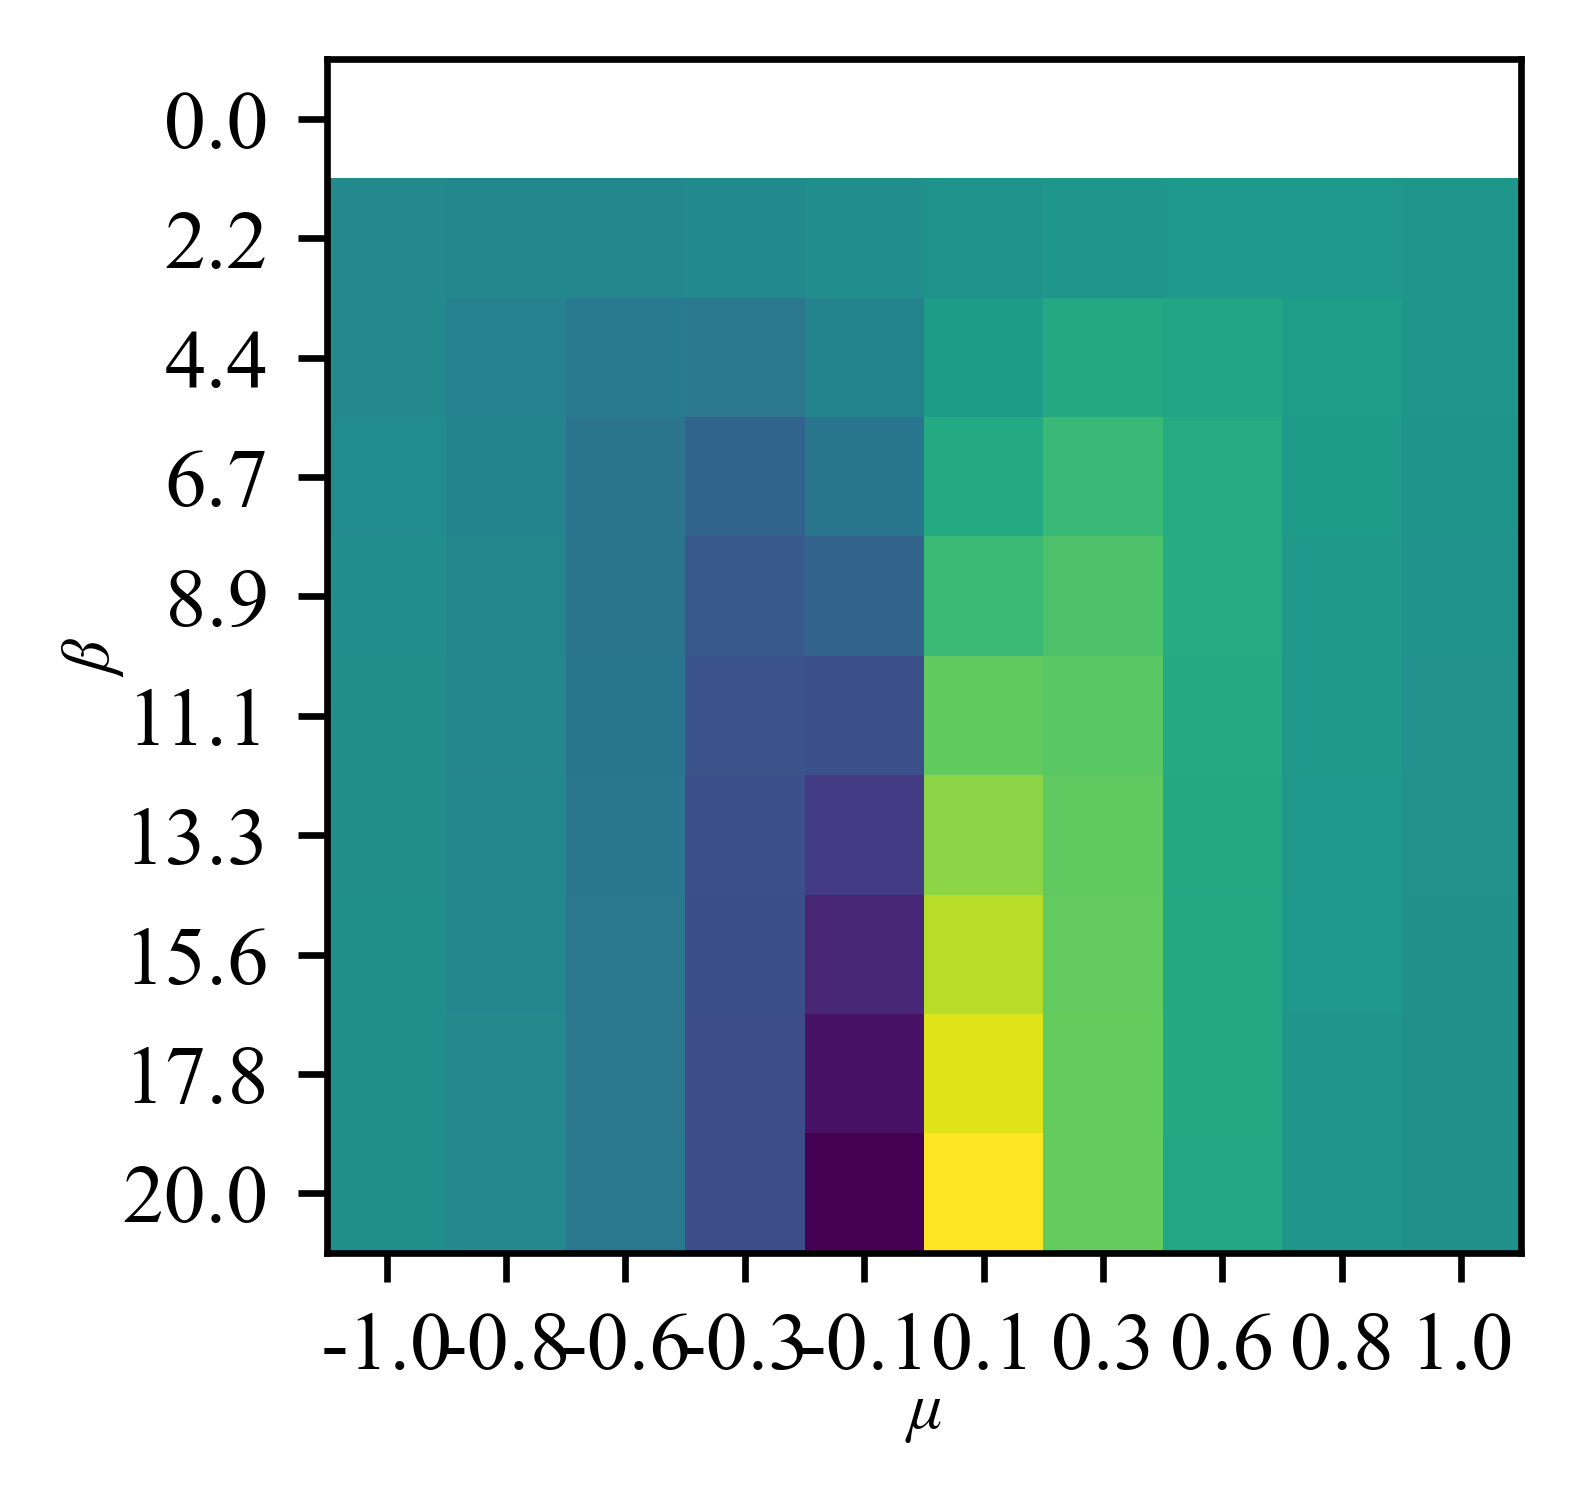
\includegraphics[keepaspectratio]{figures/muBetaPhase.png}}

}

\caption{\label{fig-muBetaPhase}Maximum deviation over range of
\(\mu,\beta\), \(f_{pre}=0.005, D=1, \epsilon=0, n=200\)}

\end{figure}%

This isn't quite the same as (Strachan, Purkayastha, and Clark 2025) fig
2, but some common features emerge. The behaviour about \(\mu=0\) is
familiar - there is a nearly discontinuous line as the max deviation
sign flips. Furthermore for lower \(\beta\) (and higher \(T\)) there is
a ``smearing'' with less extreme values. Two features differ. First of
all, Figure~\ref{fig-muBetaPhase} returns NaN for \(\beta=0\). This
isn't necessarily an issue, i suspect its just a boundary computational
effect which can be ignored for now. More importantly, (Strachan,
Purkayastha, and Clark 2025) fig 2 has symetrical ``gaps'' in max
deviation for \(\beta>7\) about \(\mu\). These aren't present in
Figure~\ref{fig-muBetaPhase}. I suspect the simulation parameters aren't
the same; Figure~\ref{fig-muBetaPhase} was produced using standard test
parameters i've been using the validate the code.

Ok quickly skimming (Strachan, Purkayastha, and Clark 2025), they use
\(f_{pre}=0.02/\pi^2 \approx 0.002\), so is less coupled than
\(f_{pre}=0.005\). This may explain why Figure~\ref{fig-muBetaPhase}
lacks this region.

Right running another dataset with that prefactor and a finer resolution
now that it seems to be working. After much anticipated waiting
(\textasciitilde20min), it has produced (a rather ugly plot):

\begin{figure}

\centering{

\pandocbounded{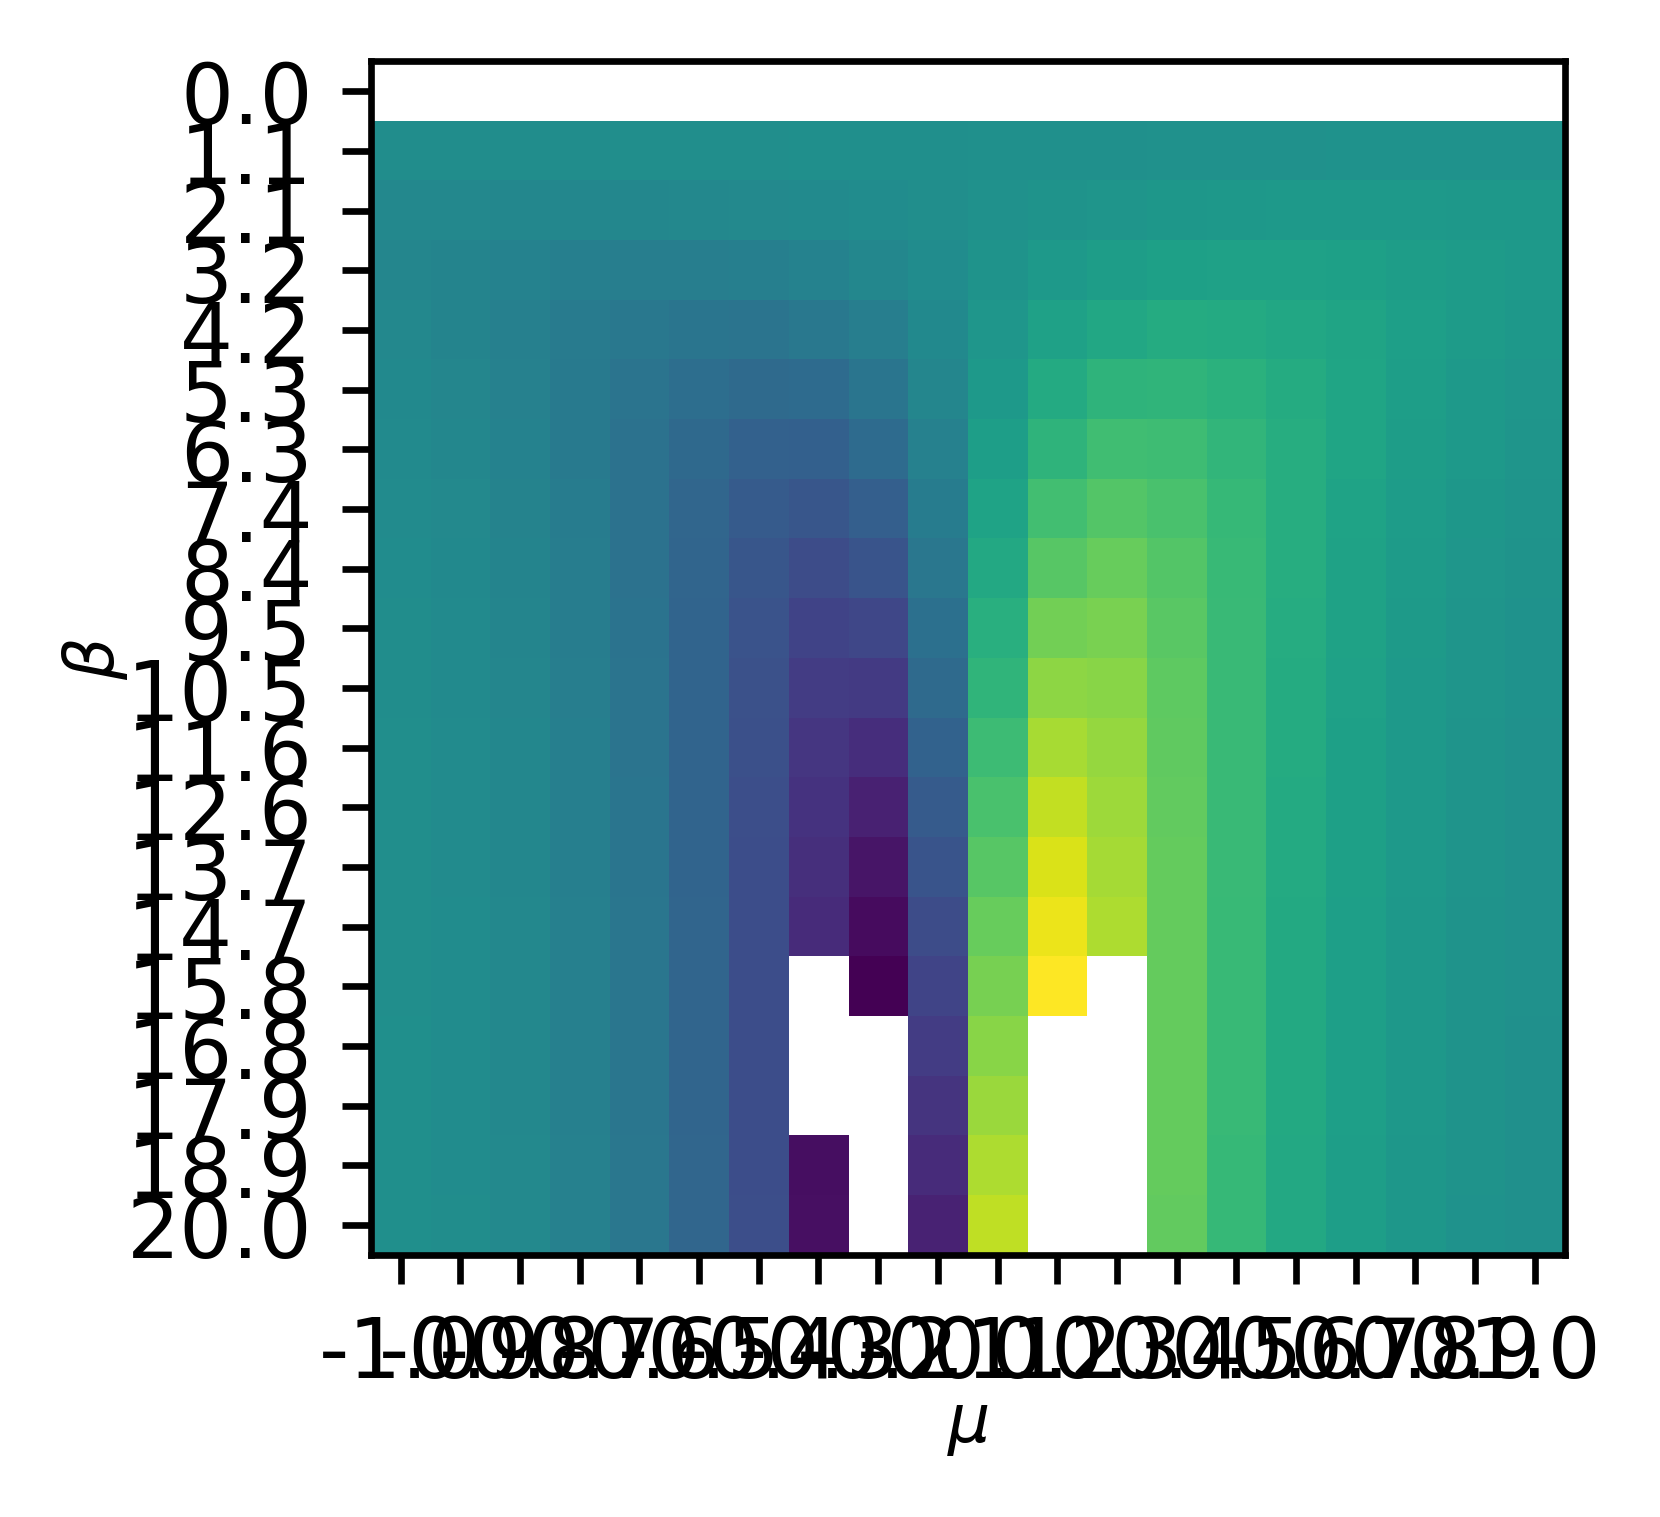
\includegraphics[keepaspectratio]{figures/muBetaPhase2.png}}

}

\caption{\label{fig-muBetaPhase2}Maximum deviation over range of
\(\mu,\beta\), \(f_{pre}=0.02/\pi^2, D=1, \epsilon=0, n=200\)}

\end{figure}%

Which not what i expected\ldots{} I strongly suspect that the gaps in
this are computing artefacts. Alternatively, these may be the same gaps
as in (Strachan, Purkayastha, and Clark 2025), but incomplete for
whatever reason. A thing which may cause issues is the relatively long
timestep \(\Delta t=1\) - this makes for a rather coarse time evolution
which may obscure the actual maximum deviation value. Additionally, the
sims aren't running for particularly long (\(t_{max}=50\)), therefore
the numerical thermalization may not be converging properly, skewing the
results. I'm unsure how this would affect the data\ldots{} Not a today
problem, will discuss this w/supervisors tmr.

\subsection{11/11/2026}\label{section-1}

\subsubsection{Supervisor meeting}\label{supervisor-meeting}

\begin{itemize}
\tightlist
\item
  analytically relate kernel to map - try to gt idea of what it
  represents
\item
  implement kernel
\item
  reaction coords - expanding system to inc bath sites
\item
  lack of gaps in Figure~\ref{fig-muBetaPhase} are expected - slightly
  different measure to in paper
\end{itemize}

To do list:

\begin{itemize}
\tightlist
\item
  Continue as planned

  \begin{itemize}
  \tightlist
  \item
    can connect the expression for the map to the kernel directly
  \item
    impleent the kernel method
  \end{itemize}
\end{itemize}

Some longer term ideas discussed:

\begin{itemize}
\tightlist
\item
  potentially explore the correlations w/bath more explicitly; these are
  source of memory, so may be useful in later analysis
\item
  maybe expand system to include a bath site - reaction coords -
  expanding system to inc bath sites - (The reaction coordinate mapping
  in quantum thermodynamics)
\end{itemize}

\subsection{15/11/2026}\label{section-2}

Right, two things to do before next meeting. I think i'm going to
implement the kernel first. Its the somewhat more ``straightforward''
step and the one which will produce more results. Quickly resumarising
some stuff from Wk3, the TTM method recursively builds the memory kernel
as:

\begin{equation}\phantomsection\label{eq-transferTensorTransform2}{
T_{k} = \Lambda_{k}-\sum_{j=1}^{k}T_{j}\Lambda_{k-j}
}\end{equation}

w/the propagation following:

\begin{equation}\phantomsection\label{eq-tensorPropagation}{
\rho(t_{k}) = \sum_{j=1}^{k}T_{j}\rho(t_{k-j})
}\end{equation}

With the dynamic map expressed as:

\begin{equation}\phantomsection\label{eq-mapCorrelationForm2}{
\hat{\Lambda(t)} = \begin{bmatrix}
1-C_{unocc}(t) & 1-C_{unocc}(t) \\
C_{unocc}(t) & C_{occ}(t)
\end{bmatrix}
}\end{equation}

Right implementation has gone quickly/smoothly, however am unsure what
these objects represent. It spits out a 2x2 matrix (which makes sense
given Equation~\ref{eq-transferTensorTransform2}), so it may be worth
doing the derivation.

Have simply plugged in Equation~\ref{eq-mapCorrelationForm2} (and
substituted \(c_{unocc}(t)=c_{0}(t_{k})\), \(c_{occ}(t)=c_{1}(t_{k})\)
for convenience) into Equation~\ref{eq-transferTensorTransform2}:

\begin{equation}\phantomsection\label{eq-tensorMapRelation}{
\begin{align}
T_{k} &= \begin{bmatrix} a_{k} & b_{k} \\ c_{k} & d_{k} \end{bmatrix} \\
a_{k}&=1-c_{0}(t_{k})-\sum_{j=1}^{k}a_{j}+c_{0}(t_{k-j})(b_{j}-a_{j}) \\
b_{k}&=1-c_{0}(t_{k})-\sum_{j=1}^{k}a_{j}(1-c_{0}(t_{k-j}))+b_{j}c_{1}(t_{k-j}) \\
c_{k}&=c_{0}(t_{k})-\sum_{j=1}^{k}c_{j}+c_{0}(t_{k-j})(d_{j}-c_{j}) \\
d_{k}&=c_{1}(t_{k})-\sum_{j=1}^{k}c_{j}(1-c_{0}(t_{k-j}))+d_{j}c_{1}(t_{k-j}) \\
\end{align}
}\end{equation}

There is evidently structure in Equation~\ref{eq-tensorMapRelation};
intuition indicates that \(T_{k}\) may be expressable in terms of 2
parameters, although thats a hunch\ldots{} Doing some rearanging, the
variables \(v_{k}=a_{k}+c_{k}\) and \(w_{k}=b_{k}+d_{k}\) may be useful?
These can be expressed as:

\begin{equation}\phantomsection\label{eq-tensorMapSubstitution1_v}{
v_{k}=a_{k}+c_{k}=1-\sum_{j=1}^{k}v_{j}(1-c_{0}(t_{k-j}))+w_{j}c_{0}(t_{k-j})
}\end{equation}

\begin{equation}\phantomsection\label{eq-tensorMapSubstitution1_w}{
w_{k}=b_{k}+d_{k}=1+c_{1}(t_{k})-c_{0}(t_{k}) - \sum_{j=1}^{k}v_{j}(1-c_{0}(t_{k-j}))+w_{j}c_{1}(t_{k-j})
}\end{equation}

hmmm, not sure thats the best substitution to make\ldots{} Would be nice
to get the eigenvectors of Equation~\ref{eq-tensorMapRelation}, however
that promises to be horrible to compute, so want to avoid that for
now\ldots{}

Going to work through Equation~\ref{eq-tensorPropagation}, \(\rho\) has
intuitive physical meaning, so this may provide insight into the terms
in \(T_{k}\):

\begin{equation}\phantomsection\label{eq-tensorPropagationSubstitution1}{
\begin{align}
\rho(t_{k})&=\sum_{j=1}^{k}T_{j}\rho(t_{k-1}) \\
&=\sum_{j=1}^{k}\begin{bmatrix}a_{j} & b_{j} \\ c_{j} & d_{j}\end{bmatrix}\begin{bmatrix}1-p(t_{k-j}) \\ p(t_{k-j})\end{bmatrix} \\
&=\sum_{j=1}^{k}\begin{bmatrix}a_{j}+(b_{j}-a_{j})p(t_{k-j}) \\ c_{j}+(d_{j}-c_{j})p(t_{k-j}) \end{bmatrix} \\
\begin{bmatrix}1-p(t_{k}) \\ p(t_{k})\end{bmatrix} &= \sum_{j=1}^{k}\begin{bmatrix}a_{j}+(b_{j}-a_{j})p(t_{k-j}) \\ c_{j}+(d_{j}-c_{j})p(t_{k-j}) \end{bmatrix}
\end{align}
}\end{equation}

Given the interelated terms in \(\rho\),
Equation~\ref{eq-tensorPropagationSubstitution1} can be interelated as:

\begin{equation}\phantomsection\label{eq-tensorPropagationSubstitution1_relation}{
\begin{align}
p(t_{k}) &= 1 - \sum_{j=1}^{k} a_{j}+(b_{j}-a_{j})p(t_{k-j}) \\ 
p(t_{k}) &=\sum_{j=1}^{k} c_{j}+(d_{j}-c_{j})p(t_{k-j}) \\
\downarrow \\
1&=\sum_{j=1}^{k}(a_{j}+c_{j})+(b_{j}+d_{j}-a_{j}-c_{j})p(t_{k-j}) \\
&= \sum_{j=1}^{k}v_{j}+(w_{j}-v_{j})p(t_{k-j})
\end{align}
}\end{equation}

Which may be a useful identity\ldots{} I think it can be reduced further
as:

\begin{equation}\phantomsection\label{eq-tensorPropagationSubstitution1_relationIdentity}{
\begin{align}
1&= \sum_{j=1}^{k}v_{j}+(w_{j}-v_{j})p(t_{k-j})\\
\sum_{j}^{k}\frac{1}{k} &= \sum_{j=1}^{k}v_{j}+(w_{j}-v_{j})p(t_{k-j}) \\
\frac{1}{k} &= v_{j}+(w_{j}-v_{j})p(t_{k-j}) \\
\downarrow k\to\infty \\
0 &= v_{j}+(w_{j}-v_{j})p(t_{k-j}) \\
\end{align}
}\end{equation}

I'm unsure if this is a valid thing to do; particularly the
\(k\to\infty\) limit. Furthermore i'm not quite sure what this
represents; it encodes some sort of constraint on \(T_{k}\), however its
unclear what sort of constraint\ldots{} I wonder if substituting in
dynamically propagated \(\rho(t)=\Lambda\rho(0)\) into
Equation~\ref{eq-tensorPropagationSubstitution1} may be helpful\ldots{}

Not a today thing\ldots{}

\phantomsection\label{refs}
\begin{CSLReferences}{1}{0}
\bibitem[\citeproctext]{ref-DavidMpemba2026}
Strachan, David J., Archak Purkayastha, and Stephen R. Clark. 2025.
{``Non-{Markovian} {Quantum} {Mpemba} {Effect}.''} \emph{Physical Review
Letters} 134 (22): 220403.
\url{https://doi.org/10.1103/PhysRevLett.134.220403}.

\end{CSLReferences}




\end{document}
